\documentclass{article}
\documentclass{article}
%%
%% Author: maciejsrokowski
%% 17/07/2018
%%

% Preamble
\documentclass[11pt]{article}

% Packages
\usepackage{a4wide}
\usepackage{amsmath}
\usepackage{physics}
\usepackage{siunitx}
\usepackage{graphicx}
\usepackage{cancel}

% Document
\begin{document}

    \title{Matrices}
    \maketitle

    \newtheorem{theorem}{Theorem}
    \newtheorem{definition}{Definition}
    \newtheorem{example}{Example}
    \newtheorem{problem}{Problem}


    \section{Matrix multiplication}

    \begin{example}
        \begin{align*}
            \begin{cases}
                u_1 =2x_1 +3x_2 + 3x_3 \\
                u_2 = 2x_1 + 4x_2 + 5x_3 \\
                u_3 = x_1 + x_2 + 2x_3
            \end{cases}
        \end{align*}
        We can express this as a matrix product, or specifically a dot product between rows of A and columns of X
        \begin{align*}
            A\vdot X & =U\\
            \bmqty{2 & 3 & 3\\
            2 & 4 & 5\\
            1 & 1 & 2}
            \bmqty{x_1 \\ x_2 \\ x_3 }
            & =\bmqty{u_1 \\ u_2 \\ u_3}
        \end{align*}
    \end{example}

    \subsection{1 \cross n and n \cross 1 Matrices}
    Two special kinds of matrices are \textbf{row vector}: the 1 \cross n matrices and \textbf{column vectors}: n \cross 1
    \section{Matrix operations}
    There are four basic operations which produce new matrices from old
    \begin{itemize}
        \item 1. Scalar multiplication\\
        Multiply each entry by $c: cA=(ca_{ij})$
        \item 2. Matrix addition\\
        Add the corresponding entries:$A + B = (a_{ij} + b_{ij})$; the two matrices must have the same number of rows and the same number od columns.
        \item 3. Transposition\\
        The transpose of the $m \cross n$ matrix A is the $n \cross m$ matrix obtained by making the rows of A the columns of the new matrix. Common notations for the transpose are $A^T$ and $A^\prime$; using first we can write its definition as $A^T = (a_{ij)})$
    \end{itemize}

    \section{Matrix multiplication}\\
    This is the most important operation. Schematically, we have\\

    \begin{align*}
        & A & \vdot & B & = C\\
        & m \cross n & & n \cross p & m \cross p\\
        & & & c_{ij} & = \sum_{k=1}^n a_{ik}b{kj}
    \end{align*}

    \subsection{Laws and properties of matrix multiplication}
    \begin{itemize}
        \item M-1. Distributive laws\\
        $A(B + C) = AB + AC$
        \item M-2. Associative laws\\
        $(AB)C = A(BC)$
        \item M-3. Existence of \textbf{Identity Matrix} such as $AI=A$ and $IA=A$. It has ones on its diagonal axis and zeros elewhere\\
        \begin{equation}
            I_3 = \pmqty{ 1 & 0 & 0 \\
            0 & 1 & 0 \\
            0 & 0 & 1}
        \end{equation}
        \item M-4. Not commutative
        \item M-5. Determinant law for two square matrices on $n \cross n$\\
        \begin{equation}
            \abs{AB} = \abs{A}\abs{B}\text{, also written } \det{AB}=\det{A}\det{B}
        \end{equation}
        \item M-6. We can simply pick out a column or a row of any matrix by a vector with all zeros and one 1\\
        \begin{equation}
            \bmqty{1 & 2 & 3\\
            4 & 5 & 6 \\
            7 & 8 & 9}
            \bmqty{0 \\ 1 \\ 0}
            =\bmqty{2 \\ 5 \\ 8}
        \end{equation}
        \begin{equation}
            \bmqty{1 & 0 & 0}
            \bmqty{1 & 2 & 3\\
            4 & 5 & 6\\
            9 & 8 & 9}
            =\bmqty{1 & 2 & 3}
        \end{equation}
    \end{itemize}

    \subsection{The meaning of matrix multiplication}
    Mulitplying AB represents doing transformation B, then transformation A.\\

    \begin{example}
        Rotation in the plane by $\ang{90}$
        \begin{gather*}
            R=\bmqty{0 & -1 \\ 1 & 0}\\
            R\vu{i} = \bmqty{0 & -1 \\ 1 & 0}\bmqty{1 \\ 0} = \bmqty{0 \\ 1} = \vu{j}\\
            R\vu{j}=\bmqty{0 & -1 \\ 1 & 0 }\bmqty{0 \\ 1 } = \bmqty{-1 \\ 0 } = -\vu{i}\\
            R\bmqty{x \\ y} = \bmqty{-y \\ x}
        \end{gather*}
    \end{example}

    \begin{example}
        Rotation by $\ang{180}$ in this way is just:
        \begin{gather}
            R^2 = \bmqty{-1 & 0 \\ 0 & -1} = -I_{2\cross2}
        \end{gather}
    \end{example}

    \section{Matrix Inverses}
    Inverse of A is a matrix M such that $AM=I$ and $MA=I$. In order for this to be true A needs to be \textbf{square matrix}\\
    \begin{gather*}
        M=A^{-1}
    \end{gather*}
    Solution to $AX=b$ is $X=A^{-1}B$, proof:
    \begin{gather*}
        AX=B\\
        \text{Multiply both sides by $A^{-1} \textbf{on the left}$}\\
        A^{-1}(AX)=A^{-1}B\\
        IX=A^{-1}B\\
        X=A^{-1}B
    \end{gather*}

    \subsection{How to invert the matrix (for small matrices)}
    \begin{gather*}
        A^{-1}=\frac{1}{\det{A}}adj(A)\text{, where adj is adjoint, which is a \textbf{Transpose of a cofactor matrix}}\\
    \end{gather*}

    \begin{example}
        \begin{gather*}
            A=\bmqty{2 & 3 & 3\\
            2 & 4 & 5 \\
            1 & 1 & 2}\\
            \text{Find minors}\\
            \vmqty{3 & -1 & -2\\
            3 & 1 & -1\\
            3 & 4 & 2}\\
            \text{Find cofactors, flip signs in the checkerboard}\\
            \vmqty{3 & 1 & -2\\
            -3 & 1 & 1\\
            3 & -4 & 2}\\
            \text{Transpose to get the adjoint}\\
            \vmqty{3 & -3 & 3\\
            1 & 1 & -4\\
            -2 & 1 & 2}\\
            \text{Find determinant}\\
            \det{A}=3\\
            \text{Divide adjoint by determinant}\\
            A^{-1}=\frac{1}{3}\vmqty{3 & -3 & 3\\
            1 & 1 & -4\\
            -2 & 1 & 2}\\
        \end{gather*}
    \end{example}

    \begin{example}
        Let $A=\bmqty{3 & 1 & -1\\
        -1 & 2 & 0\\
        -1 & -1 & -1}$\\
        Solve $A\va{x}=\va{b}$ where $b=\bmqty{1 \\ 2 \\ -3}$
        \begin{gather*}
            x=A^{-1}b\\
            \text{Find inverse of A}\\
            \text{Find minors matrix}\\
            \bmqty{-2 & 1 & 3\\
            -2 & -4 & -2\\
            2 & -1 & 7}\\
            \text{Change signs to get cofactor matrix}\\
            \bmqty{-2 & -1 & 3\\
            2 & -4 & 2\\
            2 & 1 & 7}\\
            \text{transpose to get the adjoint}\\
            adj{A}=\bmqty{-2 & 2 & 2 \\
            -1 & -4 & 1 \\
            3 & 2 & 7}\\
            \text{Find determinant, can use minors or cofactor matrix for this as well}\\
            \det{A}=3(-2) - 1(1) + (-1)3 = -10\\
            \text{Find inverse A}\\
            A^{-1} = -\frac{1}{10}\bmqty{-2 & 2 & 2 \\
            -1 & -4 & 1 \\
            3 & 2 & 7}\\
            \text{Resolve $A^{-1}b$}\\
            \va{x}=-\frac{1}{10}\bmqty{-2 & 2 & 2 \\
            -1 & -4 & 1 \\
            3 & 2 & 7}\bmqty{1 \\ 2 \\ -3}
            =\bmqty{\frac{2}{5} \\
            \frac{6}{5}\\
            \frac{7}{5}
            }
        \end{gather*}
    \end{example}

    \section{Equations of planes}
    An equation for plane is of the form $ax+by+cz=d$ and defines a plane.

    \begin{example}
        Plane with normal vector N
        \begin{gather*}
            \va{N} = \bmqty{1 & 5 & 10}\\
            \text{Point P (z, y, z) is in the plane if}\\
            \va{OP}\vdot\va{N}=0\\
            x + 5y + 10z=0
        \end{gather*}
    \end{example}

    \begin{example}
        Plane through $P_0 \bmqty{2, 1, -1} \text{ and } \bot \va{N} \bmqty{1 & 5 & 10}$\\
        \begin{gather*}
            \va{P_0 P}\vdot \va{N}=0\\
            \bmaty{x-2 & y-1 & z+1}\vdot\bmqty{1 & 5 & 10}=0\\
            (x-2) + 5(y-1) + 10(z+1) = 0 \\
            x + 5y + 10z -3 = 0
        \end{gather*}
    \end{example}

    \subsection{Normal vector}
    A Normal vector is a vector that is orthogonal to the plane. It is described by the equation of the plane minus the free variable. In order to describe the plane completely we also need it's distance to the origin. We can denote it as:\\
    \begin{gather*}
        \va{N}=\bmqty{n_1 & n_2 & n_3}\\
        P = \bmqty{p_1 & p_2 & p_3}\\
        \text{Plane equation}=n_1 (x - p_1 ) + n_2 (y - p_2 ) + n_3 (z - p_3)\\
        \text{Plane equation}=n_1 x + n_2 y + n_3 z = n_1 p_1 + n_2 p_2 + n_3 p_3\\
    \end{gather*}

    \begin{problem}
        Find the equation of the plane containing the three points $P_1 = \bmqty{1 & 0 & 1}$ $P_2 = \bmqty{0 & 1 & 1}$ $P_3 = \bmqty{1 & 1 & 0}$\\
        \begin{gather*}
            \va{N} = \va{P_1 P_2} \cross \va{P_1 P_2}\\
            \va{N} = \bmqty{i & j & k\\
            -1 & 1 & 0\\
            0 & 1 & -1}
            = -i -j -k\\
            -(x - 1) -(y - 0) -(z-1)=0
        \end{gather*}
    \end{problem}

    \subsection{Distance from the plane}
    We can easily find the distance to the plane by acknowledging the following:\\
    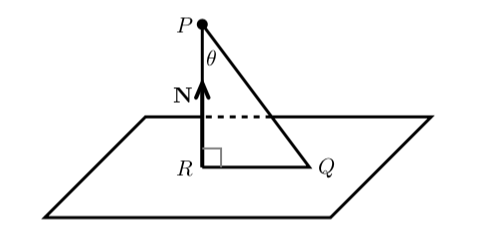
\includegraphics{fig_8.png}
    \begin{gather*}
        \text{distance}=\abs{PR} = \abs{\va{PQ}}\cos{\theta}=\abs{\va{PQ}\vdot\frac{N}{\abs{N}}}\\
    \end{gather*}
    So that means the distance is equal to dot product of the distance of the point from orgin and the normal vector and later the result of this is divided by length of the normal vector.

    \section{Linear systems}
    Linear systems are systems of equations where each of the equations describes a plane.
    \begin{example}
        \begin{align*}
            \mqty{& x & & +z & =1\\
            & x & +y & & = 2\\
            & x & +2y & +3z & = 3}
        \end{align*}\\
        All the equations describe some planes. When two planes intersect they form a line. When a plane intersects a line the result is a point. So three equations basically describe a point. This point is a solution of a linear system.\\
        Solution to $AX=B$ is given by $X=A^{-1}B$
    \end{example}
    This works fine until some planes don't intersect (for example they are parallel but at some distance from each other) or they intersect forming a line or a plane.

    \subsection{Determining solution type}
    Recall $A^{-1}=\frac{1}{\det{A}}adj(A)$\\
    We can always calculate the adjoint but what happens if the determinant is equal to zero? It means that the matrix is \textbf{NOT INVERTIBLE}. If the matrix is not invertible we cannot solve such system of equations.\\
    Geometrically situation where determinant is equal to zero is when third plane is parallel to the line at the intersection of first two planes.
    \subsection{Homogenosity}
    The linear system Ax = b is called homogeneous if b = 0; otherwise, it is called inhomogeneous
    \paragraph{Homogenous systems}
    Homogenus systems are systems where $AX=0$
    \begin{example}
        \begin{gather*}
            \mqty{x+z &=0\\
            x+y &=0\\
            x+ 2z + 3z &=0}
        \end{gather*}
        There is always the obvious solution $(0 , 0 ,0)$ also called a trivial solution. That means that all three planes pass through the origin. It has two subcases:\\
        \begin{itemize}
            \item if $\det{A} \neq 0$ we can invert A\\
            $AX=0 \leftrightarrow X=A^{-1}0=0$\\
            And that's the only solution
            \item If $\det{A}=0
            \leftrightarrow \det{\va{N_1} ,\va{N_{2} ,\va{N_3}}=0}
            \item \leftrightarrow\va{N_1}, \va{N_2}, \va{N_3} \text{ are co-planar}$\\
            This corresponds to the situation where all three normal vectors are parallel to the intersection line. They li in the same plane so the parallelepiped formed by them has volume 0. This is called a non-trivial solution\\
            In this case we have infinietly many solutions
        \end{itemize}
    \end{example}
    \paragraph{Inhomogenous systems}
    $AX=B$ for this we have three cases:\\
    \begin{itemize}
        \item if $\det{A}\neq 0 $ then unique solution is $A^{-1}B$
        \item if $\det{A}=0$ then either we have \textbf{no solutions} or \textbf{infinietly many solutions}
    \end{itemize}
    \subsection{Consistency}
    We call system consistent if it has solutions and inconsistent otherwise.
    \subsection{Singularity}
    A square matrix is called \textbf{singular} if $\abs{A}=0$ and \textbf{nonsingular} if $\abs{A}\neq 0$\\
    Even if $\abs{A} \approx 0$ the matrix is called \textbf{ill-conditioned} as it may run into troubles with numerical calculations and the solutions are very sensitive to small changes in the coefficients of A\\
    \begin{problem}
        Consider the system\\
        \begin{gather*}
            \mqty{2x & &+ cz & =4\\
            x & -y & + 2z & = \pi\\
            x & -2y & +2z & =-12}
        \end{gather*}
        Find c for which:\\
        \begin{itemize}
            \item a) there is a unique solution\\
            \begin{gather*}
                \det{A} = 4-c\\
                c\neq 4
            \end{gather*}
            \item b) the corresponding homogenous system has a unique solution\\
            For both a) and b) the answer is the same as the value of c for which this system has a unique solution are dependent only on $\abs{A}$ as the value that makes A invertible  (even though the actual solutions may be different)
        \end{itemize}

    \end{problem}
\end{document}